\chapter{ Hyperledger Fabric}
\section{Giới thiệu Hyperledger Fabric }
Hyperledger Fabric là một nền tảng blockchain phân tán được phát triển bởi Tổ chức Linux. Nó 
cung cấp một giải pháp cho các tổ chức và doanh nghiệp để triển khai các ứng dụng blockchain 
tùy chỉnh. Hyperledger Fabric được thiết kế để có tính linh hoạt và khả năng mở rộng dễ dàng, 
cho phép các thành phần của hệ thống phát triển và triển khai độc lập với nhau.

Hyperledger Fabric có tính bảo mật cao và hỗ trợ quản lý danh tính và quản lý quyền truy cập, 
giúp bảo vệ dữ liệu của người dùng trên blockchain. Nó bao gồm các hợp đồng thông minh, sổ cái và
hệ thống mà người tham gia vào hệ thống quản lý các giao dịch của họ.

Điểm khác biệt giữa Hyperledger Fabric và các nền tảng blockchain khác là:
\begin{itemize}
    \item[-] Thiết kế dựa trên mô hình module 
    \item[-] Hỗ trợ quản lý danh tính và quyền truy cập
    \item[-] Độc lập với tiền tiện tử
    \item[-] Hỗ trợ các giao thức đồng thuận kết hợp
\end{itemize}

\subsection{Mô hình module}

Hyperledger Fabric được thiết kế dựa trên mô hình module, cho phép các thành phần của hệ 
thống được phát triển và triển khai độc lập với nhau. Điều này giúp cho việc phát triển và 
triển khai các ứng dụng blockchain trở nên dễ dàng hơn.
Một Fabric tiêu chuẩn gồm các module sau:
\begin{itemize}
    \item[-] Ordering service được sử dụng để quản lý và xác nhận các giao dịch 
    trên mạng blockchain.
    
    \item[-] Membership service provider là một thành phần trong hệ thống Hyperledger Fabric, 
    được sử dụng để quản lý và xác thực danh tính trên mạng blockchain. Nó đảm bảo rằng chỉ 
    các thành viên được ủy quyền mới có thể tham gia vào mạng blockchain và thực hiện các 
    hoạt động trên đó. MSP sử dụng các chứng chỉ xác thực để xác định quyền truy cập của mỗi thành viên trong mạng.
    \item[-] Cross-chain messaging service được sử dụng để cho phép các peer khác nhau có thể 
    tương tác và giao tiếp với nhau trực tiếp, mà không cần thông qua một bên trung gian nào khác.
    \item[-] Hợp đồng thông minh chaincode được sử dụng để triển khai các hợp đồng thông minh trên blockchain.
    \item[-] Sổ cái nơi lưu trữ tất cả các thông tin về các giao dịch và trạng thái của mạng blockchain. 
    Hyperledger Fabric sử dụng một kiểu sổ cái phân tán để đảm bảo tính toàn vẹn và bảo mật của các giao dịch trên mạng. 
    
\end{itemize}

\subsubsection{Quản lý danh tính và quyền truy cập}
Hyperledger Fabric có tính năng hỗ trợ quản lý danh tính và quyền truy cập để đảm bảo 
tính bảo mật và phân quyền trong mạng blockchain. Dưới đây là một số tính năng quan trọng 
trong việc quản lý danh tính và quyền truy cập trong Hyperledger Fabric:

\begin{itemize}
    \item[-] Xác thực và ủy quyền: hỗ trợ nhiều phương thức xác thực và ủy quyền khác nhau, 
    chẳng hạn như xác thực bằng chứng chỉ SSL/TLS, xác thực bằng tài khoản và mật khẩu, 
    xác thực bằng mã thông báo truy cập (access token), và ủy quyền bằng các chứng chỉ.
    \item[-] Quản lý danh tính: cung cấp tính năng quản lý danh tính để quản lý các thông tin
    về người dùng và tổ chức trên mạng blockchain.
    \item[-] Quản lý quyền truy cập: cung cấp tính năng quản lý quyền truy cập để quản lý 
    người dùng đảm bảo rằng với mỗi người dùng có nhiệm vụ khác nhau thì quyền truy cập trong
    hệ thống là khác nhau.
    \item[-] Quản lý chứng chỉ: cung cấp tính năng quản lý chứng chỉ để quản lý các chứng chỉ
    và chứng thư số, để bảo mật và xác thực người dùng. 

\end{itemize}
\subsection{Độc lập với tiền tiện tử}

Hyperledger Fabric là một nền tảng blockchain phổ biến được thiết kế để sử dụng trong các 
ứng dụng doanh nghiệp. Khác với các tiền điện tử như Bitcoin hay Ethereum, Hyperledger 
Fabric không phải là một loại tiền điện tử và không thực hiện các giao dịch tiền tệ. Thay 
vào đó, nó cung cấp các tính năng để đảm bảo tính toàn vẹn và bảo mật của dữ liệu trong 
mạng blockchain, giúp các doanh nghiệp triển khai các ứng dụng blockchain phù hợp với nhu 
cầu của họ.

Cụ thể hơn, trong Bitcoin hay Etherem, khi miner giải bài toán khó PoW để xác minh tính
toàn vẹn của thông tin sẽ được một phần thưởng là một lượng tiền điện tử. Thay vào đó, Hyperledger Fabric
sử dụng một hệ thống đồng thuận phân cấp để đảm bảo tính toàn vẹn và bảo mật của dữ liệu 
trên mạng blockchain. Các thành viên trong mạng Hyperledger Fabric được xác định và quản 
lý bởi các chứng chỉ xác thực và quy tắc thành viên. Khi một giao dịch mới được đề xuất, 
các thành viên trong mạng sẽ thẩm định và chấp nhận nó trước khi thêm vào blockchain.

\subsection{Cơ chế đồng thuận kết hợp}
Hyperledger Fabric là một nền tảng blockchain dành cho doanh nghiệp, có khả năng hỗ trợ 
nhiều cơ chế đồng thuận khác nhau như Proof of Work (PoW), Practical Byzantine Fault 
Tolerance (PBFT) và Kafka Ordering Service. Việc sử dụng cơ chế đồng thuận kết hợp trong 
Hyperledger Fabric được thực hiện nhằm đảm bảo tính toàn vẹn và bảo mật của hệ thống. 

PBFT được sử dụng để đồng thuận giữa các peer trong mạng, đảm bảo rằng các giao dịch 
được xác nhận và thêm vào blockchain chỉ khi được chấp thuận bởi đa số các peer trong mạng. 
Bên cạnh đó, Kafka Ordering Service được sử dụng để quản lý thứ tự của các block mới được 
thêm vào blockchain, tránh xảy ra các xung đột về thứ tự của các block. 

Ngoài ra, Hyperledger Fabric cũng có thể sử dụng các cơ chế đồng thuận khác như PoW hoặc PoS 
tùy thuộc vào yêu cầu của từng ứng dụng blockchain cụ thể. 

Trình bày cụ thể về các cơ chế đồng thuận kết hợp trong Hyperledger Fabric, tôi sẽ trình bày 
ở phần \textbf{Kiến trúc hệ thống} sau khi đã trình bày cụ thể về cấu tạo của một mạng blockchain
trên Hyperledger Fabric. 
\section{Mô hình Hyperledger Fabric}
\subsection{Thành phần hệ thống}
\subsubsection{Node}
Các node trong hệ thống này đảm nhận các vai trò khác nhau. Có quyền truy cập và vai trò khác
nhau trong hệ thống.
Có 3 loại node trong hệ thống:  
\begin{itemize}
    \item[-] Peer node: Là nút mạng tham gia vào quá trình xử lý giao dịch và lưu trữ 
    dữ liệu trong mạng blockchain. Mỗi peer node có một bản sao của ledger và có 
    thể thực hiện các chức năng như giao tiếp với các node khác, xác thực và xử lý 
    giao dịch, thực hiện các chaincode (smart contract), cập nhật trạng thái của 
    ledger, và đồng bộ dữ liệu với các peer node khác.
    \item[-] Orderer node: đảm nhận vai trò đồng thuận và quản lý thứ tự của các 
    block mới được thêm vào blockchain.
    \item[-] Client node: Nó tạo và huỷ các giao dịch, đảm nhận vai trò giao tiếp với các node khác trong mạng.
       
\end{itemize}
\subsubsection{Tài sản - asset}
Asset là các đối tượng có giá trị được quản lý trên mạng blockchain trong 
Hyperledger Fabric. Mỗi asset có một ID duy nhất và được lưu trữ trong world state 
ledger. Trạng thái của mỗi asset được đại diện bởi cơ sở dữ liệu key-value và 
được cập nhật thông qua chaincode để tạo mới, cập nhật, xóa và truy vấn thông tin.
Các hoạt động này được thực hiện thông qua các giao dịch trên một Channel Ledger.
\subsubsection{Chaincode}

Trong Hyperledger Fabric, hợp đồng thông minh được gọi là chaincode. Chaincode là 
một phần mềm các định một hoặc nhiều nội dung. Nó thực thi các quy tắc được xác định
để đọc và thay đổi các cặp giá trị key-value được lưu trữ trong sổ cái. 

Một transaction proposal được gửi đến các peer node trong mạng blockchain, và các 
peer sử dụng chaincode để kiểm tra và xác minh đề xuất giao dịch này. Nếu các quy 
tắc được định nghĩa bởi chaincode được tuân thủ, giao dịch được thực thi và kết 
quả được áp dụng cho ledger trên tất cả các peer.

\subsubsection{Ledger}
Mỗi ledger là một bản sao của toàn bộ blockchain và được lưu trữ trên mỗi peer node trong mạng.
Hệ thống có thể lưu trữ nhiều ledger khác nhau, mỗi ledger được lưu trữ trên một channel riêng biệt. 
Trong Hyperledger Fabric, có hai loại ledger chính:

\begin{itemize}
    \item[-] World state ledger: Lưu trữ trạng thái hiện tại của tất cả các 
    asset (tài sản) trong mạng blockchain. World state ledger được lưu trữ dưới dạng cơ sở dữ liệu key-value (khóa - giá trị), trong đó khóa là ID của asset và giá trị là trạng thái hiện tại của asset đó.
    \item[-] Transaction log ledger: Lưu trữ toàn bộ lịch sử các giao dịch được thực hiện 
    trên mạng blockchain. Transaction log ledger bao gồm các block được kết nối theo đúng 
    thứ tự thời gian, mỗi block chứa thông tin về các giao dịch được thực hiện trong khoảng 
    thời gian đó.
\end{itemize}
\subsubsection{Channel}

Trong hệ thống Hyperledger Fabric, channel là một tính năng quan trọng để cung cấp cách thức 
truyền tải thông tin và giao tiếp bảo mật giữa các thành viên trong mạng blockchain.

Mỗi channel là một kênh truyền thông riêng biệt giữa một nhóm các thành viên trong mạng, 
cho phép các thành viên trong kênh đóng vai trò như các bên liên quan duy nhất đến các giao 
dịch và trạng thái của ledger liên quan đến kênh đó. Điều này có nghĩa là nếu một thành 
viên không thuộc kênh không có quyền truy cập vào các giao dịch và trạng thái của kênh đó.

Mỗi channel có một ledger riêng, bao gồm một World State Ledger và một Transaction Log Ledger, 
để lưu trữ thông tin về trạng thái hiện tại của ledger và lịch sử các giao dịch liên quan đến 
ledger đó. Khi một giao dịch được thực hiện trên một channel, nó sẽ chỉ ảnh hưởng đến ledger 
của channel đó và không ảnh hưởng đến các channel khác.

Một peer có thể tham gia cùng lúc nhiều channel là lưu trữ tất cả các ledger của các channel.


\subsection{Luồng giao dịch trong Hyperledger Fabric}

Luồng giao dịch có các bước sau:
\begin{figure}[h]
    \centering
    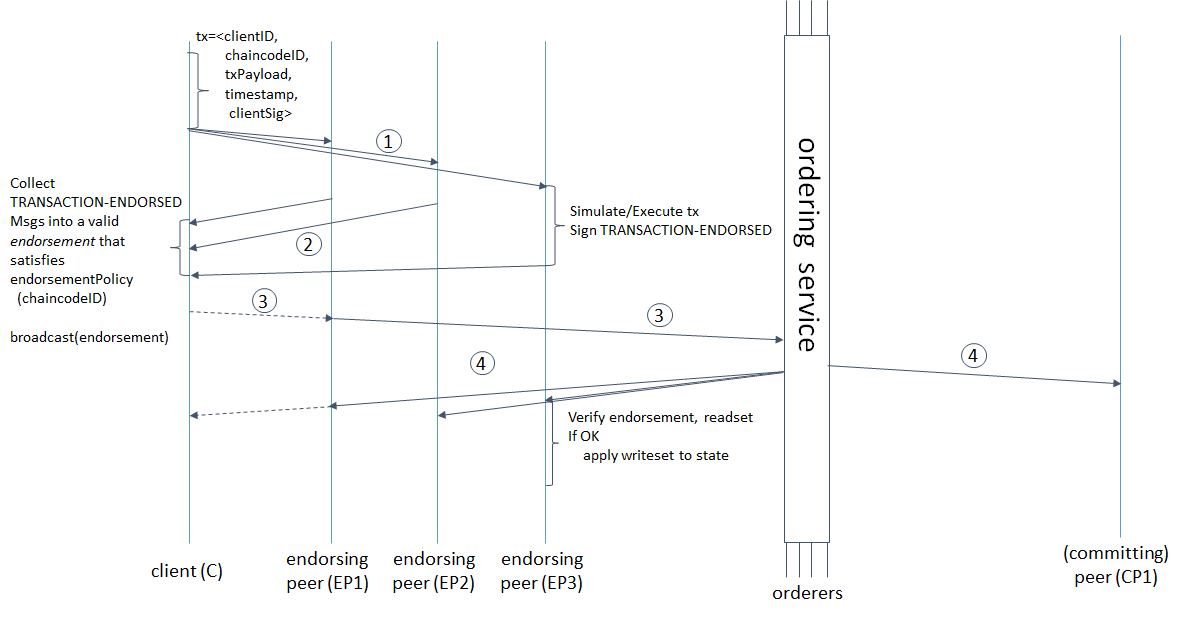
\includegraphics[width=1\textwidth]{images/flow-4.png}
    \caption{Luồng giao dịch }
\end{figure}


\begin{itemize}
    \item[\textbf{1.}] Client gửi một giao dịch đến các endorsing peer node. Endorsing peer node là 
    một nút trong mạng blockchain Hyperledger Fabric, được sử dụng để chứng nhận tính hợp 
    lệ của một giao dịch trước khi nó được gửi đến các nút khác để xác nhận và cam kết trên 
    sổ cái. Nó không lưu trữ trực tiếp các thông tin liên quan đến giao dịch hoặc sổ cái.
    \item[\textbf{2.}] Khi một giao dịch được gửi đến endorsing peer, nó sẽ thực hiện một số hoạt 
    động để chứng nhận tính hợp lệ của giao dịch đó. Đầu tiên, endorsing peer node sẽ kiểm 
    tra xác thực của người gửi giao dịch và xác định xem họ có quyền thực hiện giao dịch hay 
    không. Sau đó, endorsing peer sẽ thực hiện việc thực thi các hàm chaincode để xác 
    định xem giao dịch có hợp lệ hay không. Với mỗi một lệnh được thực hiện thì ta ghi lại 
    trạng thái đọc và ghi của dữ liệu,gọi là tập ReadWrite RW
    Nếu endorsing peer thấy là giao dịch hợp lệ, nó sẽ tạo một chữ ký bảo lãnh (endorsement signature) và gửi lại cho người 
    gửi giao dịch. 
    \item[\textbf{3.}] Khi một giao dịch được chứng nhận hợp lệ, người gửi giao dịch sẽ gửi giao dịch
    đó đến các ordering service. Các ordering node sẽ xác định thứ tự của các block dựa trên 
    chữ ký bảo lãnh của các endorsing peer và sắp xếp các giao dịch vào các khối tương 
    ứng. Sau đó nó gửi các block đến cac peer.
    \item[\textbf{4.}] Committing peer sẽ xác nhận lại các chính sách xác thực một lần nữa. 
    Đồng thời nó kiểm tra hiệu lực của tập RW. Việc xác nhận giao dịch sẽ được lưu vào World- state, còn sổ cái sẽ lưu lại các giao dịch. Khi này, sổ cái được đồng bộ hóa.
\end{itemize}
